\chapter{Prototyp urządzenia}
\label{cha:prototyp}

Głównym zagadnieniem pracy było stworzenie kompletnego urządzenia, które wykryje niebezpieczne zdarzenie i poinformuje o tym zdefiniowanego użytkownika. W niniejszym rozdziale, przeprowadzono testy, mające pomóc stworzyć odpowiednie algorytmy. Opisano również kolejne kroki procesu tworzenia urządzenia, a także rozważono różne podejścia w rozwiązaniu problemów. Omówione zostały również poszczególne fragmenty działającego urządzenia.

Tę część pracy, rozpoczęto od przeprowadzenia podstawowych eksperymentów, mających pokazać, jakich przyspieszeń można spodziewać się w przypadku rzeczywistego zderzenia na rowerze. Testy, rozpoczęto od stworzenia urządzenia, mającgo zbierać surowe dane z akcelerometru. Ze względu na łatwość i szybkość implementacji, wykorzystano platformę Raspberry Pi Zero W, z systemem operacyjnym Raspbian Lite. Korzystając z gotowch bibliotek, napisany został skrypt, który po uruchomieniu tworzył plik tekstowy, do którego zapisywał surowe dane, pobrane z akcelerometru. Sam akcelerometr, ustawiony był na częstotliwość próbkowania 416Hz i skalę $\pm$8g.
\newline
Ze względów czysto praktycznych, tj. w celu zabezpieczenia płytek przed uszkodzeniem, wykonany został model 3D prostej obudowy, który następnie wydrukowano na drukarce 3D. Rysunek \ref{img:test_device_a} przedstawia Raspberry w wykonanej na potrzeby projektu obudowie. Zgodnie z rysunkami technicznymi płytki, wykorzystano otwory montażowe. Następnie, stworzono dodatkową warstwę izolacyjną między płytkami, do której przymontowano płytkę z akcelerometrem.(Rysunek \ref{img:test_device_b}) Gotowy układ, zasilany był przy użyciu powerbanku, połączonego przez USB. Obudowa, zamknięta była drukowaną pokrywką. Rozwiązanie przedstawia rysunek \ref{img:test_device_c}.
\newline


\section{Opracowanie algorytmu wykrywania kolizji}
Cały układ, zasilany był przy użyciu zewnętrznej baterii, zamontowanej na siodełku roweru. Ze względu na bezpieczeństwo, testy przeprowadzane były na rowerze bez rowerzysty. Sam układ, zamontowany został na rurze podsiodłowej. Ponieważ jest to prawie centralny punkt roweru, przewidziano, że przyspieszenia w przypadku silnego wyrzucenia koła w powietrze, będą mniejsze. Eksperyment przeprowadzono przez rozpędzanie roweru do  prędkości około 1$\frac{m}{s}$ i kolejno:
\begin{itemize}
    \item Zderzenie roweru z drzewem
    \item Upadek na kamieniach
    \item Upadek ze stromego zbocza
\end{itemize}
%TODO: Podmienić zdjęcie urządzenia testowego
\begin{figure}[h]
    \centering
    \begin{subfigure}{3.5cm}
        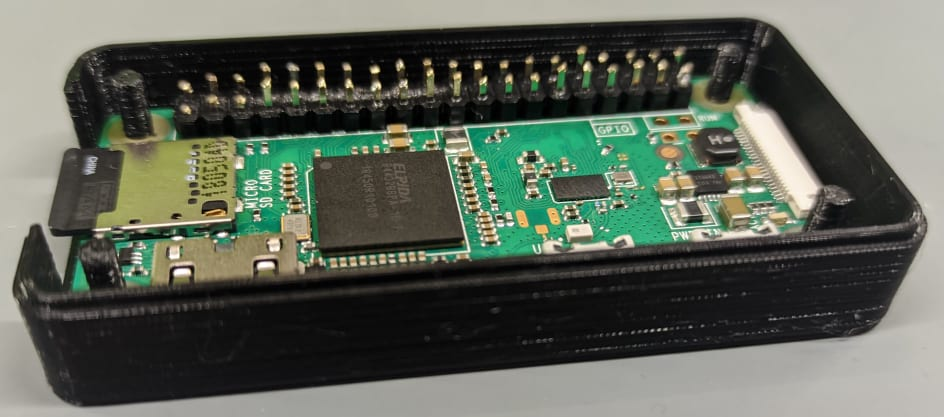
\includegraphics[width=7cm, angle=-90]{Graphics/pi.jpg}
        \caption{Raspberry Pi Zero w drukowanej obudowie}
        \label{img:test_device_a}
    \end{subfigure}
    \begin{subfigure}{3.5cm}
        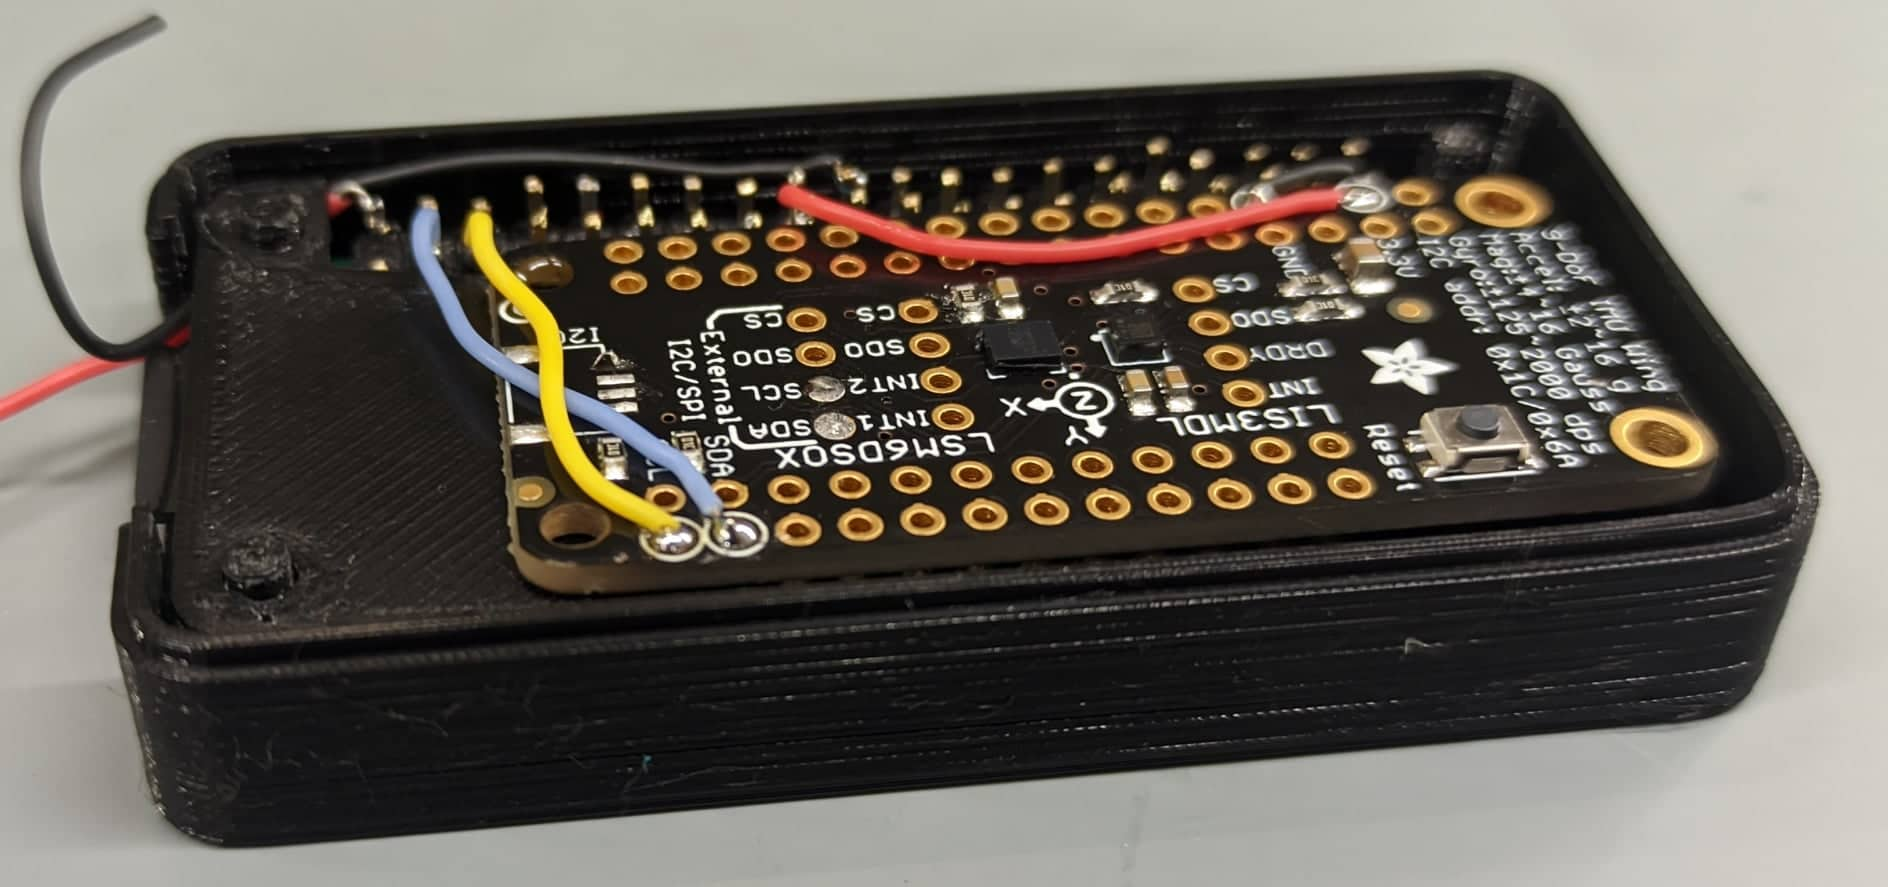
\includegraphics[width=7cm, angle=-90]{Graphics/Pi_acc.jpg}
        \caption{Płytka z akcelerometrem w obudowie}
        \label{img:test_device_b}
    \end{subfigure}
    \begin{subfigure}{3.5cm}
        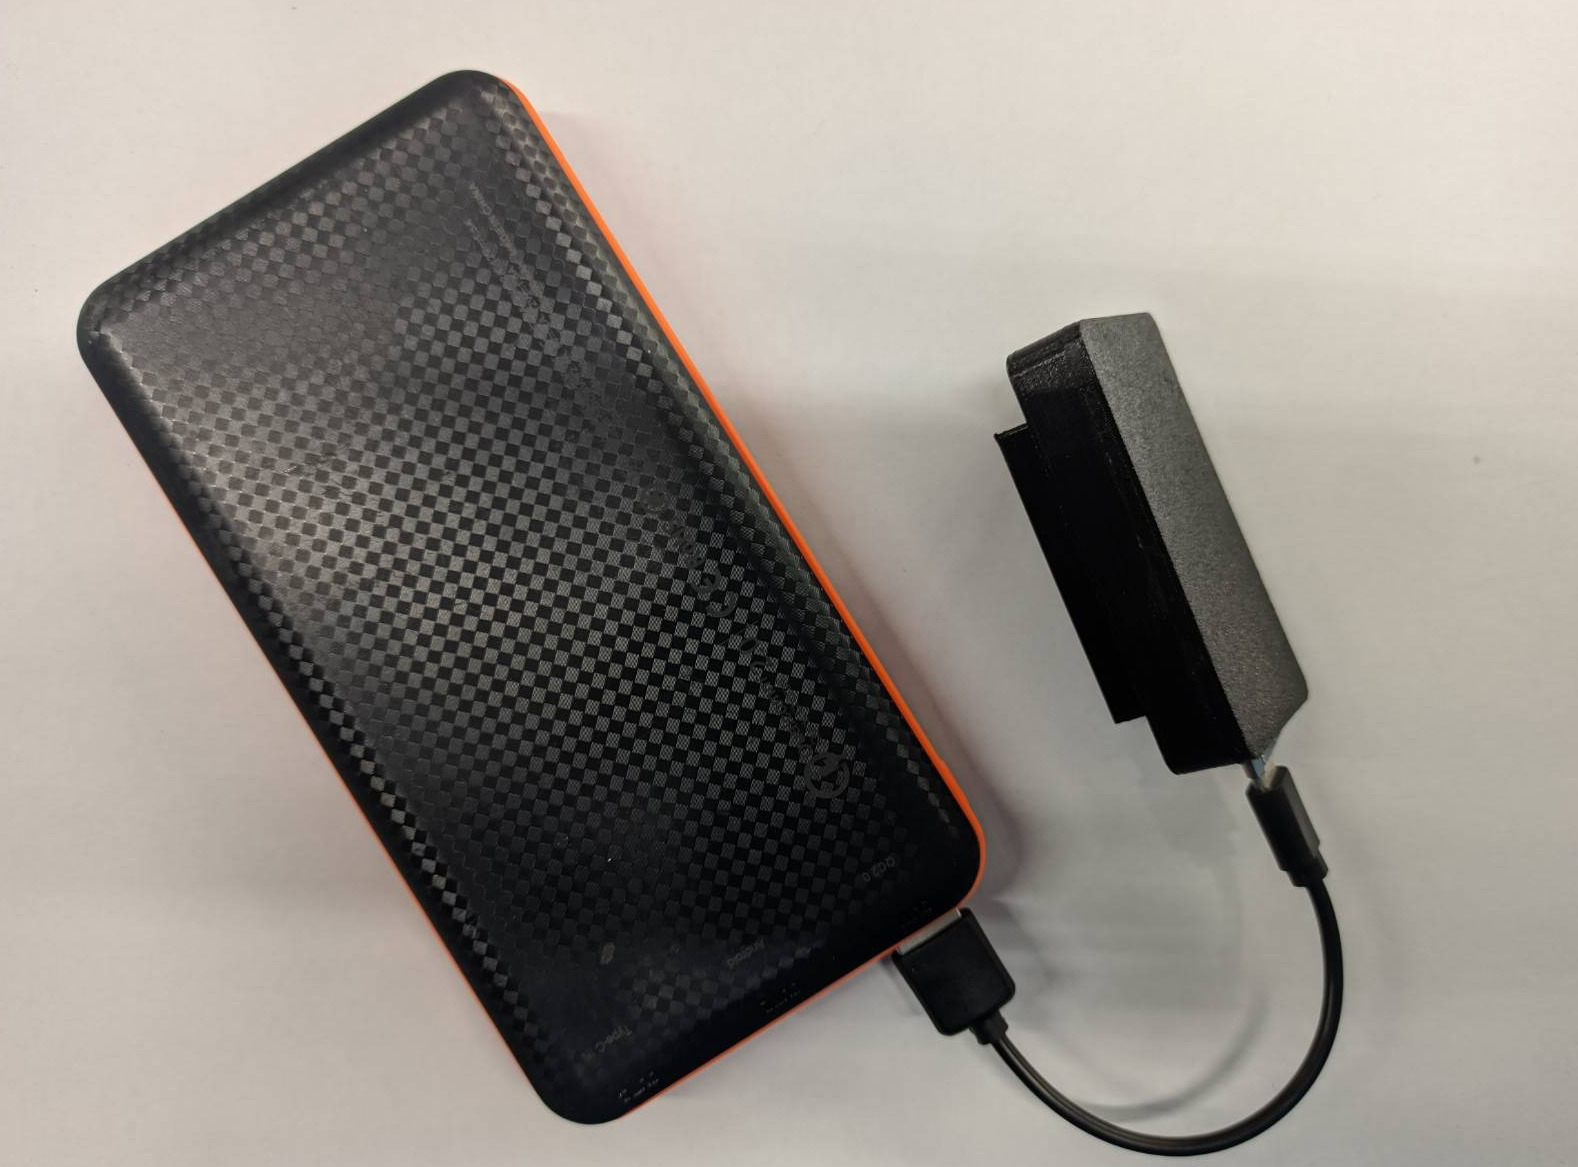
\includegraphics[width=7cm, angle=-90]{Graphics/test_device.jpg}
        \caption{Urządzenie testowe zasilane zewnętrzną baterią}
        \label{img:test_device_c}
    \end{subfigure}
    \caption{Urządzenie testowe do zbierania danych}
\end{figure}

\subsection{Analiza zebranych danych }
\label{sec:data_analysis}
W celu analizy danych, stworzono prosty skrypt w języku Python. Pobierał on surowe dane z pliku, przetwarzał, a następnie rysował zależności czasowe $a(t)$ dla każdej z osi. Ponieważ akcelerometr zwraca liczbę 16-bitową ze znakiem, należało uwzględnić ten fakt w konwersji, gdyż Python posiada dynamiczne typy danych, co mogło zakłamać wyniki. Zebrane dane, okazały się być znacząco zaszumione. Z tego powodu, przefiltrowane zostały filtrem dolnoprzepustowym. Rysunek \ref{img:bike} przedstawia orientację urządzenia na rowerze. W trakcie analizy danych, przyjęto zaznaczone na nim kierunki osi.
\begin{figure}[hb]
    \centering
    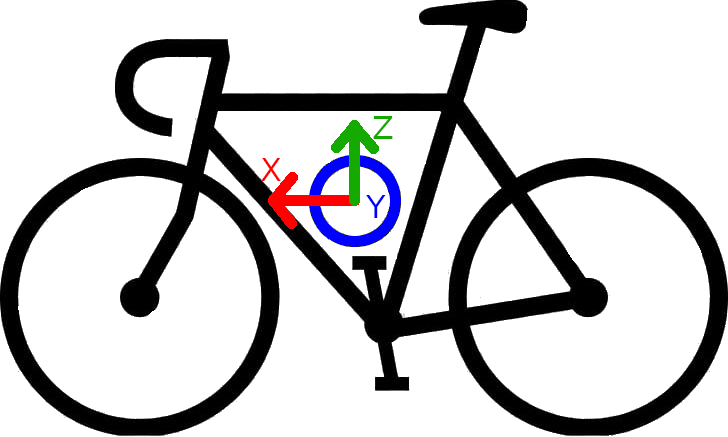
\includegraphics[width=8cm]{Graphics/rowerek.png}
    \caption{Orientacja urządzenia zamontowanego na rowerze}
    \label{img:bike}
\end{figure}
Podczas każdego z testów, rower z przymocowanym urządzeniem, rozpędzono do około 1$\frac{m}{s}$. Zgodnie z przewidywaniami, w większości przypadków przefiltrowane przyspieszenia układu sięgały ok. 1g. Należało również zwrócić uwagę na zwroty przyspieszeń, które zmieniały się po obrocie roweru. Poniżej przedstawiono trzy analizowane przebiegi, na podstawie których utworzone zostały algorytmy. 
\newline
\newline
Rysunek \ref{img:slope} przedstawia zapis upadku ze stromego zbocza. Jest to przypadek gdy rowerzysta górski podczas uskoku, traci kontrolę nad rowerem, lub wypada z trasy. Przez około pół sekundy rower swobodnie spadał, powoli przechylając się w kierunku przedniego koła. Około szóstej sekundy uderzył nim o zbocze, co widać wyraźnie zarówno na osi X, jak i Z. Następnie odbity rower ponownie uderzył w ziemię, tym razem pochylając się po odbiciu na bok. Kolejne uderzenie, było więc uderzeniem bocznym, widocznym jako głęboki dół  na osi Y. Niemal natychmiast, rower obrócił się kołami do góry, co widać na osi Z jako przyspieszenie równe -1g. Po siódmej sekundzie rower zaczął sunąć bokiem wzdłuż zbocza i szybko wyhamowywać. akcelerometr zarejestrował to jako oscylajcje na osi Y pomiędzy 7, a 8 sekundą. Na wykresie, można było również zauważyć, że po zdarzeniu, rower zatrzymał się na jednym z boków, ponieważ oś Y miała stałą wartość bliską 1g.
\newline
\newline
Kolejny z rysunków (\ref{img:stones}), przedstawia sytuację gdy rowerzysta jadąc po kamieniach, uderza tylnym kołem o jeden z nich i traci kontrolę nad rowerem. Sytuacja ta charakterysuje się silnymi oscylacjami osi X i Z, przy względnie stabilnej osi Y. W czwartej sekundzie, rower uderzył tylnym kołem w kamień. Koło zostało wyrzucone do góry, z przyspieszeniem około 1g. Po 500ms rowerzysta rower uderzył z całą energią przednim kołem w ścieżkę, osiągając przyspieszenie prawie 2g. W tej chwili pojazd testowy jeszcze raz odbił się od, a następnie bokiem uderzył w drzewo przy scieżce.
\newline
\newline
Rysunek \ref{img:tree} przedstawia sytuację, gdy rowerzysta tracąc kontrolę nad rowerem, uderza w drzewo. W tym przypadku rower po około 4.5s uderza w drzewo, co odczytane zostało jako wzrost do 0.5g na osi X. Niestety, nie było to uderzenie czyste, ponieważ duża część energii rozłożyła się na odbicie roweru od drzewa. Zapis osi Y pokazuje, że po uderzeniu, rower zaczął obracać się. Ostatecznie jednak, zatrzymał się na jednym z boków.
\newline
\newline
Przeprowadzone testy, pozwoliły na sprawdzenie przeciążeń działających na rower w trakcie wypadku. Pierwszym z nasuwających się wniosków był fakt, że niepotrzebnie ograniczona została częstotliwość próbkowania akcelerometru. W przypadku Raspberry Pi, magistrala I$^{2}$C, pozwala na transmisję 12,5kB/s. Ponieważ jeden zestaw danych zawierał 12 bajtów, częstotliwość próbkowania mogła wynosić aż 1kHz. Tymczasem, ustawiona została częstotliwość 416Hz. Ustawienie to wynikało z obawy, że kod w języku skryptowym nie nadąży za większą częstotliwością. Kolejnym z wniosków, była konieczność stosowania filtrów dolnoprzepustowych. Surowe zapisy z akcelerometru, były silnie zaszumione, na co również wpływ mogła mieć mała częstotliwość próbkowania względem szybkości zmian podczas wypadku. Mimo tego, testy dostarczyły cennych danych na podstawie których stworzono algorytmy, opisane w podrozdziale \ref{sec:state_machines}

%%%%%%%%% Zapisy upadku - wykresy %%%%%%%%%%
\begin{figure}[H]
    \centering
    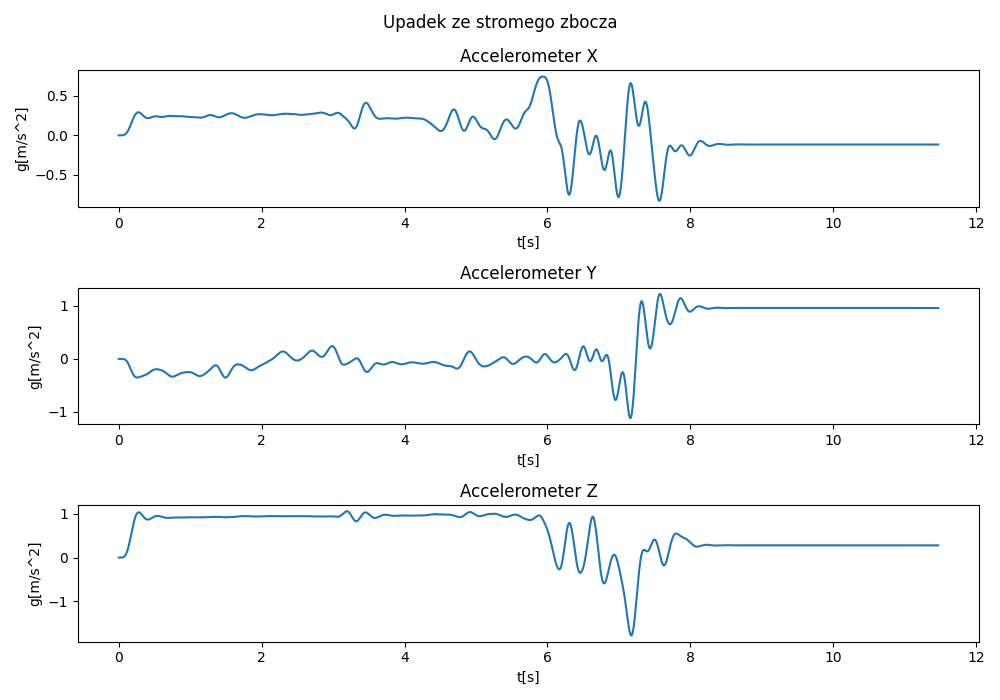
\includegraphics[width=15cm]{Graphics/slope_title.png}
    \caption{Przefiltrowany zapis upadku roweru ze stromego zbocza}
    \label{img:slope}
    \vspace{0.5cm}
    \centering
    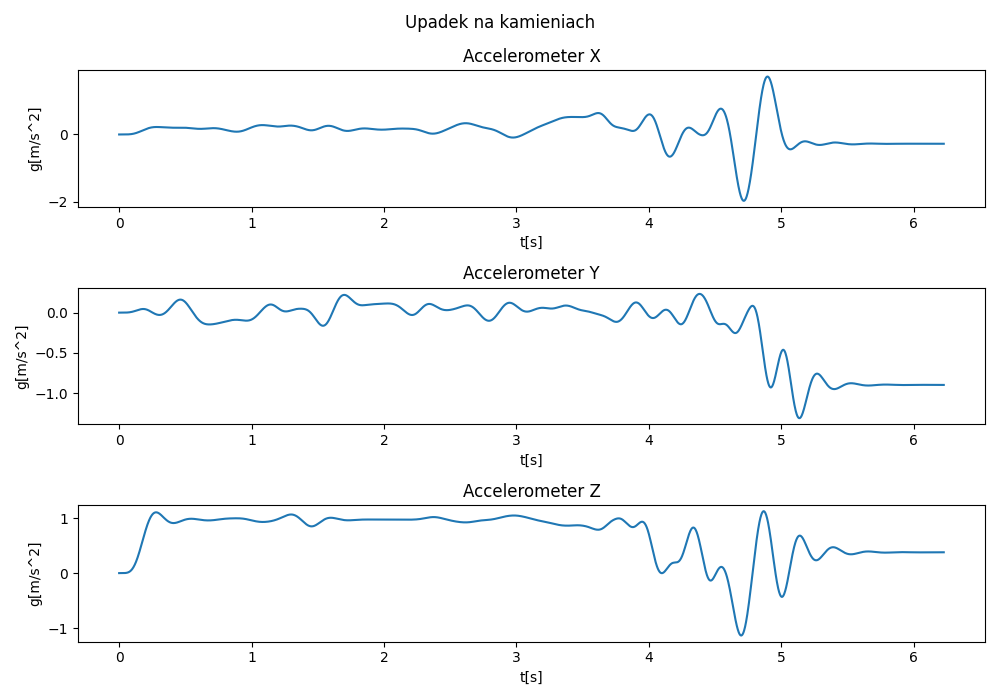
\includegraphics[width=15cm]{Graphics/Stones_title.png}
    \caption{Przefiltrowany zapis upadku roweru na kamieniach}
    \label{img:stones}
\end{figure}
\begin{figure}[h]
    \centering
    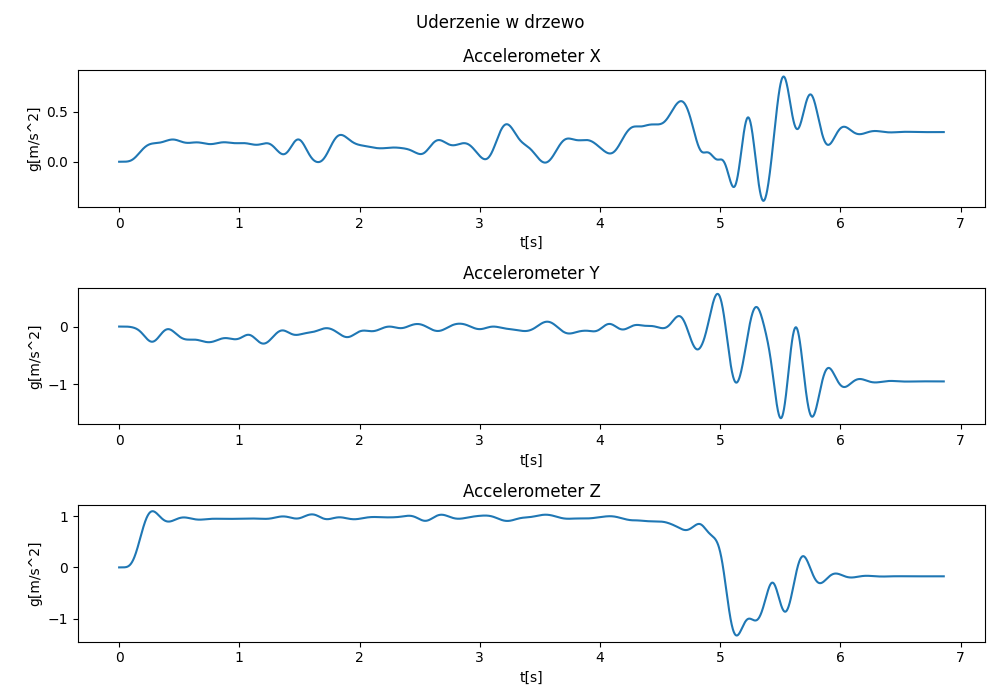
\includegraphics[width=15cm]{Graphics/Tree_title.png}
    \caption{Przefiltrowany zapis uderzenia roweru w drzewo}
    \label{img:tree}
\end{figure}

\subsection{Maszyny stanów wykrywające wypadek}
\label{sec:state_machines}
Na podstawie analizy danych z podrozdziału \ref{sec:data_analysis} zdecydowano się na implementację czterech, niezależnych maszyn stanów. Każda z nich, odpowidać będzie analizowanym przypadkom. Istotnym elementem pracy było możliwie największe uproszczenie maszyn, aby przyspieszyć działanie układu i zminimalizować zużycie energii, bez utraty skuteczności.
\subsubsection{Wykrywanie przeciążenia w dowolnej osi}
Pierwsza z maszyn stanów, służy wykryciu znaczących przeciążeń na dowolnej z osi. Podczas testów zauważono, że podczas każdego z wydarzeń, wysoka wartość przeciążenia odróżnialna była od szumu na podstawie czasu trwania. Określono, że jeśli po około 50ms próbka utrzymuje wysoką wartość, to nastąpiło silne przeciążenie. Ponieważ zdecydowano się skorzystać z wbudowanych w akcelerometr maszyn stanów, można było skorzystać z ich wewnętrznych liczników. Opisywana maszyna stanów, gdy dowolna z osi przekroczy wartość $\pm$6g, ustawia licznik na 50ms. Gdy przez ten czas, nie wystąpi próbka o wartości mniejszej niż 6g, wyzwolony zostaje alarm. Duża wartość przyspieszenia, pozwoliła uniknąć fałszywych alarmów podczas bezkolizyjnej jazdy. Maszynę przedstawia diagram \ref{img:fsm1}.
\newline
\newline
\subsubsection{Maszyna stanów wykrywająca przewrócony rower}
Dwie kolejne maszyny stanów, przedstawione na diagramie \ref{img:fsm2}, to algorytmy wykrywające przewrócenie roweru. Podczas analizy danych zauważono, że każdy wypadek, kończył się przechyleniem roweru na jeden z boków. Z tego powodu, zaimplementowano licznik, który co 2 sekundy próbkuje wartość na osi Y i sprawdza, czy przekroczyła ona wartość bezwzględną 0.6g. Jeśli przez dwie minuty, rower nie wróci do pozycji jazdy (|Y| < 0.6g), wyzwolony zostaje alarm. W praktyce, opisana maszyna musiała zostać zaimplementowana w akcelerometrze jako dwie, niezależne, z uwagi na brak funkcji wartości bezwzględnej w układzie.
\begin{figure}[h]
    \centering
    \begin{subfigure}[b]{5cm}
    \centering
    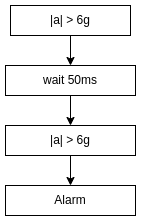
\includegraphics[width=3.5cm]{Graphics/All_axis_FSM1.png}
    \caption{Wykrycie silnego przeciążenia}
    \label{img:fsm1}
    \end{subfigure}%
    \hspace{1cm}
    \begin{subfigure}[b]{5cm}
    \centering
    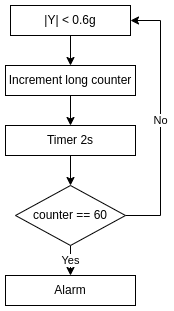
\includegraphics[width=4cm]{Graphics/overturned_FSM2_3.png}
    \caption{Wykrycie przewrócenia roweru}
    \label{img:fsm2}
    \end{subfigure}
    \caption{Maszyny 1-3}
\end{figure}
\subsubsection{Maszyna stanów wykrywająca uderzenie i upadek}
Ostatnia z maszyn stanów (rysunek \ref{img:fsm4}), wykrywa uderzenie w osi Z, czyli np. najechanie na korzeń. Następnie, przez 60 sekund sprawdza, czy rower nie wrócił do wyjściowej pozycji, czyli zwykłej jazdy. W przypadku, gdy przez 10 sekund rower nie powróci do pionu, uruchomiony zostanie alarm. Maszyna ta, okazała się być najdokładniejszą z prezentowanych. Wynika to bezpośrednioz faktu, że oś Z jest osią najbardziej stabilną w trakcie jazdy. Pozostałe maszyny, stanowią więc jej uzupełnienie.
\begin{figure}[h]
    \centering
    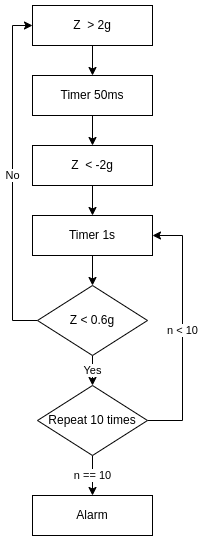
\includegraphics[width=4cm]{Graphics/Z_axis_FSM.png}
    \caption{Czwarta maszyna stanów}
    \label{img:fsm4}
\end{figure}

\section{Opracowanie logiki urządzenia}

\subsection{Wysokopoziomowy algorytm działania urządzenia}
Głównym zagadnieniem budowy urządzenia, było maksymalne wydłużenie czasu pracy na baterii. Z tego powodu, założono, że lokalizacja oraz połączenie z siecią, będą zestawiane tylko w momencie wystąpienia wypadku. Na podstawie rozważań oraz testów przeprowadzonych w podrozdziale \ref{sub:recognize-choice}, zdecydowano się na wykorzystanie maszyny stanów wbudowanej w akcelerometr. Dzięki temu, możliwym było ustawienie urządzenia w tryb głębokiego uśpienia, tuż po inicjalizacji urządzenia.
Rysunek \ref{img:app_logic} obrazuje założoną logikę urządzenia. Po uruchomieniu układu, inicjalizowane są wszystkie komponenty. W przypadku LTE, wykonywana jest rejestracja do sieci. Ponieważ jest to urządzenie odpowiedzialne za bezpieczeńswo, rejestracja przy uruchomieniu może wykryć nieprawidłowości jak brak środków na koncie, brak karty SIM czy urwana antena modemu. Ta funkcjonalność, nie została jednak zaimplementowana na tym etapie rozwoju urządzenia. Po inicjalizacji podzespołów, wyłączony został zarówno modem oraz moduł GPS. Zgodnie z założeniami, są one uruchamiane w momencie wystąpienia alarmu, aby oszczędzić energię. Kolejnym krokiem, jest wgranie zrzutu pamięci akcelerometru, celem ustawienia maszyn stanów. Po jego wykonaniu, mikrokontroler przechodzi w tryb uśpienia. W tle, uruchomiony pozostaje stos Bluetooth, pozwalając połączyć się z urządzeniem i wpisać numer telefonu, na który wysłane zostanie powiadomienie. Wyzwolenie dowolnej z maszyn stanów, uruchamia przerwanie. Wyzwolenie przerwania, skutkuje uruchomieniem modułu GPS, a po poprawnym pobraniu lokalizacji, również modemu. Powiadomienie, jest wysyłane periodycznie, do momentu wyłączenia alarmu przyciskiem. Pomiędzy alarmami, wszystkie podzespoły pozostają wyłączone, celem oszczędzania anergii.
\begin{figure}[h]
    \centering
    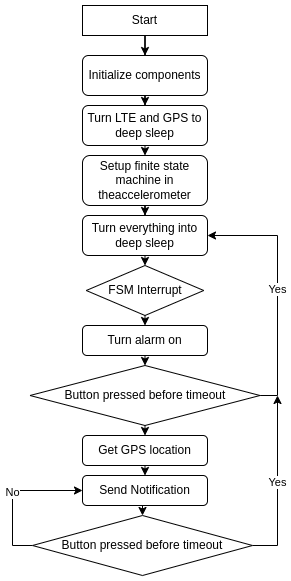
\includegraphics[width=6cm]{Graphics/APP_logic.png}
    \caption{Diagram przedstawiający logikę działania urządzenia}
    \label{img:app_logic}
\end{figure}
%%%%% Accel %%%%%
\subsection{Wybór metody analizy danych przez urządzenie}
\label{sub:recognize-choice}
Ponieważ jednym z najważniejszych elementów pracy, było osiągniecie jak najniższego zużycia energii, zdecydowano się na porównanie podejścia klasycznego, opartego na czytaniu danych i ich analizie przez mikrokontroler, z maszynami stanów realizowanymi przez akcelerometr. W tym celu, skonfigurowano prosty algorytm, wykrywający obrót urządzenia w osi Z. Akcelerometr ustawiono w tryb niskiego zużycia energii, a następnie wprowadzono mikrokontroler w tryb uśpienia. W tym stanie, układ oczekiwał na przerwanie, informujące o gotowości danych. Po jego wystąpieniu, następowało zczytanie danych z akcelerometru, a następnie porównanie ich do zdefiniowanej stałej. Po spełnieniu warunku obrotu o 180$^{\circ}$, ustawiano licznik na 2 sekundy, resetujący stan maszyny. Jeśli w tym czasie, odczytano dane o przeciwnym znaku, maszyna stanów uznana była za zrealizowaną, o czym informowano przez wiadomość wypisaną na UART. Całość, zobrazowana jest na diagramie \ref{img:recognize}.

\begin{figure}[h]
    \centering

    \begin{subfigure}[b]{5cm}
    \centering
    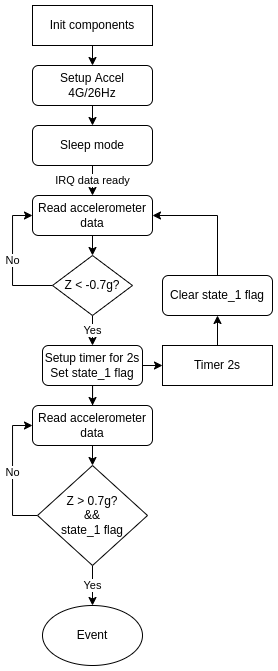
\includegraphics[width=5cm]{Graphics/Recognize_in_code.png}
    \caption{Wykrywanie zdarzenia przez mikrokontroler}
    \end{subfigure}%
    \hspace{3cm}
    \begin{subfigure}[b]{5cm}
    \centering
    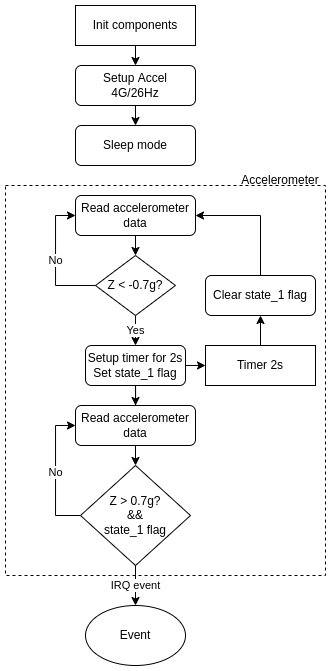
\includegraphics[width=5cm]{Graphics/Recognize_in_code_acc.png}
    \caption{Wykrywanie zdarzenia przez akcelerometr}
    \end{subfigure}%
    \caption{Analiza zdarzenia przez mikrokotroler lub akcelerometr}
    \label{img:recognize}
\end{figure}
Każde rozwiązań, zostało zmierzone przy użyciu urządzenia Otii. Jest to urządzenie służące do precyzyjnej analizy energii pobieranej przez układ \cite{otii}. Na zapisie z programu(rys. \ref{img:recognize_mcu}) wyraźnie widać inicjalizację modemu LTE, który w trakcie przeprowadzania testów był już zintegrowany na płyce PCB. Jest ona widoczna w postaci znaczącego wzrostu pobieranego przez układ prądu, sięgającego nawet 200mA. Gdy modem przechodzi w tryb głębokiego uśpienia, wyraźnie widać odczyty i przerwania, w postaci drobnych pików. Sam skok, wynikał z wywołania funkcji logującej, jednak w wyraźny sposób zaznaczał moment wystąpienia przerwania. W przypadku tego podejścia, pobór prądu wyniósł 1.58mA. Należy jednak zaznaczyć, że zastosowana tutaj maszyna stanów, była maszyną bardzo prostą. Jej rozbudowa, wiązałaby się z bardzo szybkim wzrostem zużycia energii. Kolenym z minusów była ilość generowanych przez akcelerometr przerwań. Każdy odczyt danych nie tylko zajmuje linię danych I$^{2}$C, ale również czas procesora. 
\begin{figure}[h]
    \centering
    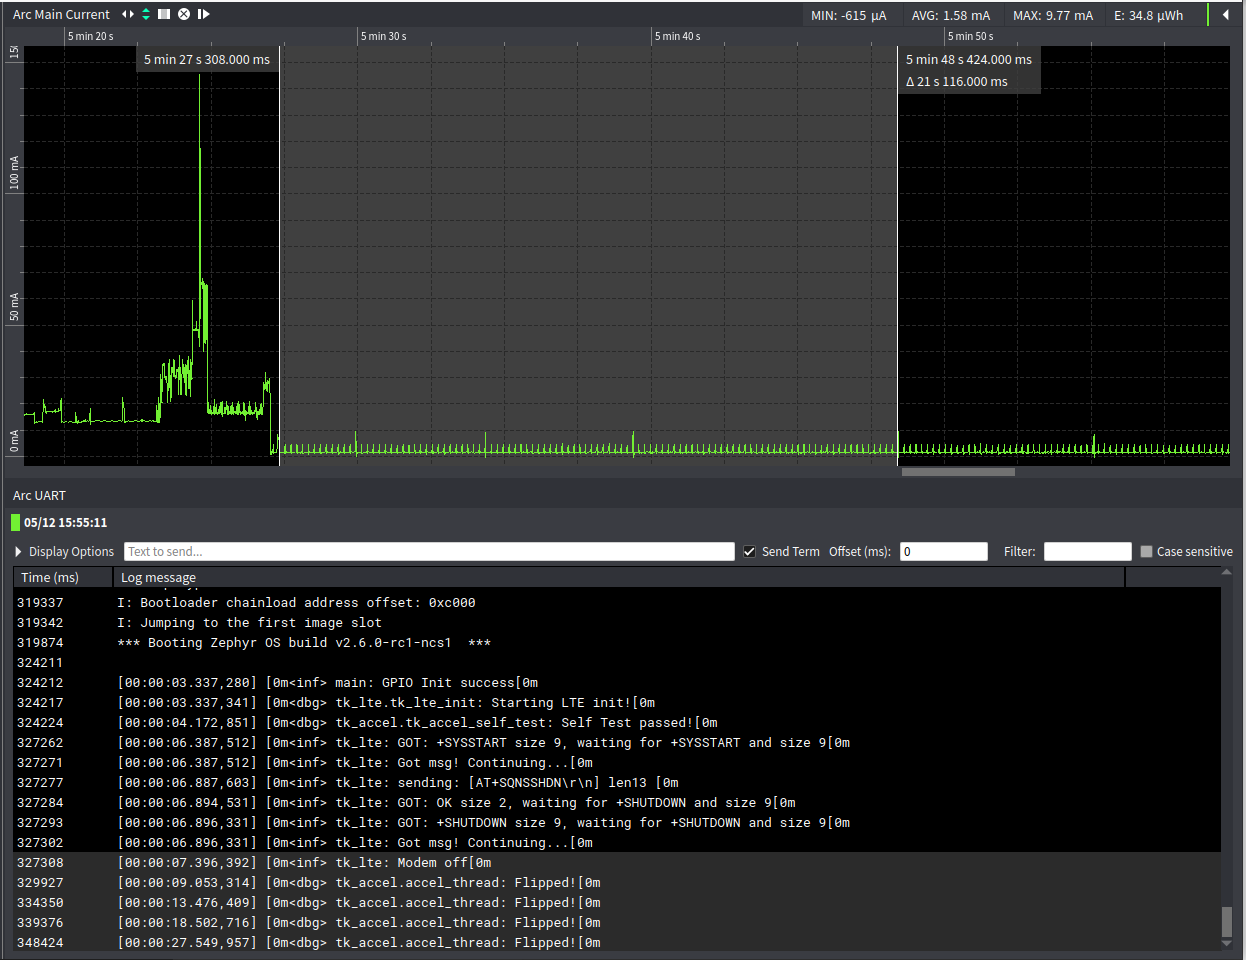
\includegraphics[width=15cm]{Graphics/recognize_mcu.png}
    \caption{Pobór prądu w czasie, podczas analizy przez mikrokontroler}
    \label{img:recognize_mcu}
\end{figure}
\newline
Podejście drugie, z maszyną stanów skonfigurowaną na akcelerometrze, okazało się zużywać średnio aż o 200$\mu$A mniej. Tak duża różnica, przy tak prostej funkcjonalności, była silnym argumentem za wykorzystaniem wbudowanej maszyny stanów. Dodatkowo, na rysunku \ref{img:recognize_acc} widać, że zniknęły gęste piki prądu. Wynikało to wprost z tego, że akcelerometr wystawia przerwanie tylko wtedy, gdy spełniona wykonana zostanie cała maszyna stanów.
\begin{figure}[h]
    \centering
    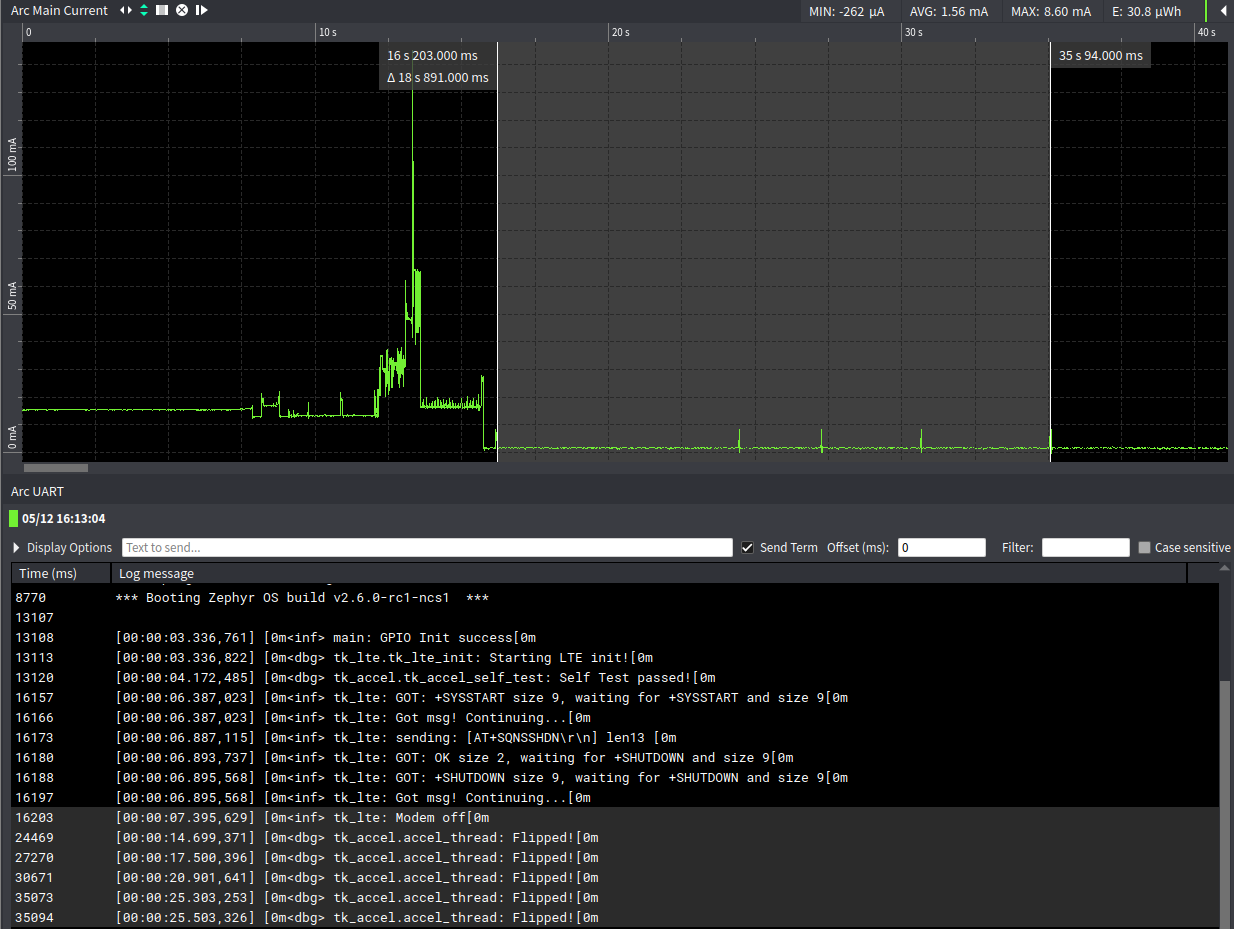
\includegraphics[width=15cm]{Graphics/recognize_acc.png}
    \caption{Pobór prądu w czasie, podczas analizy przez akcelerometr}
    \label{img:recognize_acc}
\end{figure}
Powyższe rozważanie, pokazało więc zasadność stosowania akcelerometru analizującego dane niezależnie od mikrokontrolera. Dodatkowo, STMelectronics, stworzyło zestaw narzędzi, ułatwiających budowę urządzeń, w oparciu o ich układy. Przykładem jest program Unico-GUI\cite{unico}, pozwalający programować akcelerometry w oparciu o płytki rozwojowe. Podczas tworzenia tej pracy, wykorzystano zestaw STEVAL-MKI109V3 + STEVAL-MKI197V1. Program Unico, pozwala projektować maszyny stanów w oparciu o interfejs graficzny. Było to znaczące ułatwienie, ze względu na możliwość zapisania zrzutu pamięci akcelerometru do kodu w języku C. Dzięki temu, w łatwy sposób można było testować różne konfiguracje układu, unikając ręcznego nadpisywania rejestrów. Pomocną okazała się również nota aplikacyjna, wyjaśniająca sposób, w jaki maszyny stanów powinny być programowane \cite{lsm6dsoxappnote}. Na rysunku \ref{img:unico_ss} pokazano zrzut programu, przedstawiąjący ustawienie maszyny stanów numer 1.
\begin{figure}[h]
    \centering
    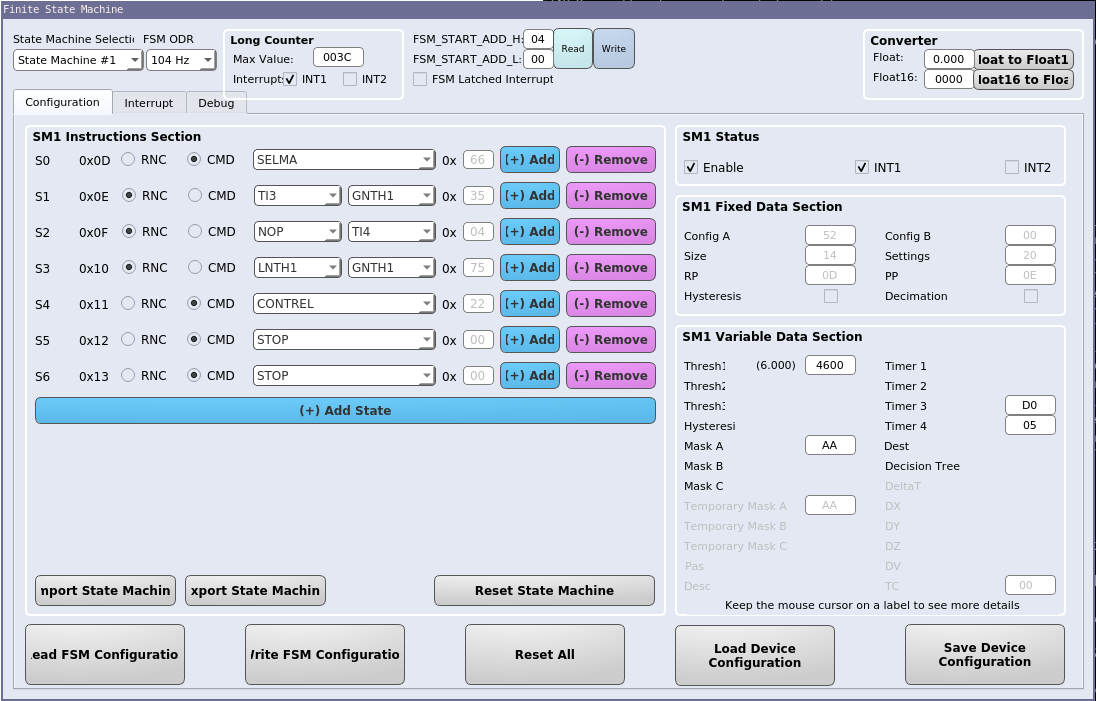
\includegraphics[width=12cm]{Graphics/unico_screenshot.png}
    \caption{Zrzut programu Unico-GUI. Implementacja maszyny stanów numer 1}
    \label{img:unico_ss}
\end{figure}
%%%%% GPS %%%%%
\subsection{Implementacja pobierania lokalizacji}
Zasada działania modułu MT3333 jest stosunkowo prosta. Zgodnie z dokumentacją\cite{MT3333}, należało w odpowiedniej kolejności uruchomić przetwornice układu, zachowując właściwe odstępy czasowe. Gdy zostaną one uruchomione poprawnie, układ zacznie szukać lokalizacji, jednocześnie cały czas wysyłając wiadomości NMEA. Wyzwaniem okazało się tutaj parsowanie przychodzących wiadomości. Ostatecznie, do bufora dopisywane były bajty, do momentu otrzymania znaku nowej linii. Przychodzące linie były testowane przez algorytm. Po otrzymaniu wiadomości zawierającej lokalizację, wiadomość parsowana była do struktury, zawierającej szerokość i wysokość geograficzną w postaci tablic bajtów. Po otrzymaniu lokalizacji, moduł był wyłączany, aby nie marnować energii. Schemat działania, przedstawiono na diagramie \ref{img:gps_diagram}.
\begin{figure}[h]
    \centering
    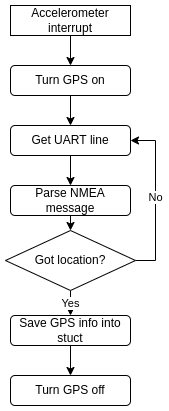
\includegraphics[width=4cm]{Graphics/GPS_NMEA.png}
    \caption{Działanie modułu GPS}
    \label{img:gps_diagram}
\end{figure}

%%%%% LTE %%%%%
\subsection{Implementacja powiadamiania o zdarzeniu}
Dzięki zastosowaniu układu SKY66430, podczas tworzenia prototypu, przetestowano dwa, zupełnie różne podejścia do problemu powiadamiania:
\begin{itemize}
    \item Zapytanie HTTP
    \item Powiadomienie SMS
\end{itemize}
Każde z podejść, zakładało logikę, przedstawioną na rysunku \ref{img:lte_diagram}. Całość komunikacji z modemem, realizowana była przy użyciu komend AT. Ważnym problemem, była kolejność wysyłanych do niego poleceń. Z tego powodu, zaimplementowana została funkcja oczekująca na odpowiedź od modemu, potwierdzającą przetworzenie wysłanej komendy. Dzięki jej zastosowaniu, zminimalizowana została szansa niepowodzenia transmisji, ponieważ w przypadku zbyt długiego oczekiwania, modem był resetowany przeznaczonym do tego pinem.
\begin{figure}[t]
    \centering
    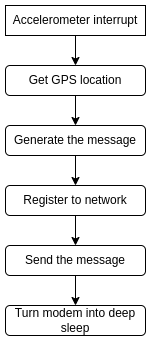
\includegraphics[width=4cm]{Graphics/LTE.png}
    \caption{Procedura wysłania powiadomienia o zdarzeniu}
    \label{img:lte_diagram}
\end{figure}

Na potrzeby przetestowania zapytań HTTP, stworzone zostało proste gniazdo TCP w JavaScript. Następnie, wykorzystując gotowe biblioteki, zaprogramowano bota na platformę Discord. Jest to platforma oparta o otwarty kod źródłowy, na której użytkownicy tworząc kanały głosowe i tekstowe, komunikują się w zorganizowany sposób. Bot, jest wirtualnym użytkownikiem, wykonującym zaprogramowane akcje. Mogą one obsługiwać specjalne funkcje serwera, lub monitorować zachowanie użytkowników. W omawianym podejściu, bot mógł wysłać powiadomienie z otrzymaną lokalizacją, do wszystkich użytkowników serwera. Ponieważ platforma posiada bardzo dobrze rozwiniętą aplikację mobilną, powiadomienie mogłoby być szybko odczytane przez jednego z użytkowników. Jednocześnie, nie byłoby wymagane definiowanie jednego, numeru docelowego. Ostatecznie jednak, rozwiązanie to zostało uznane za niepasujące do urządzenia na tym etapie. Takie podejście, wymagało stworzenia stabilnego kodu zewnętrznej aplikacji (bota). Jednocześnie, zapytanie HTTP przesyła dużo danych, w porównaniu do SMS. Mogło to okazać się problemem w miejscach o słabym zasięgu.
\newline
Finalnie, zdecydowano się na wysłanie prostego powiadomienia tekstowego, przy użyciu wiadomości SMS. Za tym rozwiązaniem, przemawiała stabilność i niezawodność sieci komórkowych, mających obecnie niemal całkowite pokrycie, nawet w górach. Wysłanie SMS, pozwoliło również uniezależnić urządzenie od innych aplikacji.
Ponieważ współrzędne geograficzne, nie są szczególnie użyteczne bez mapy, wysyłane powiadomienie SMS zawiera zawiera link do map Google. Link ten jest tworzony w kodzie układu, wykorzystując funkcje bibliotek standardowych. Rysunek \ref{img:notification} przedstawia powiadomienie, wysyłane przez urządzenie. Numer telefonu, na który powinno zostać wysłane powiadomienie, wpisywany jest do urządzenia przy użycu Bluetooth. W przypadku, gdy użytkownik nie wpisze żadnego numeru, urządzenie wyśle powiadomienie na ostatni znany mu numer. Jeśli pamięć przeznaczona na numer telefonu będzie pusta, w trakcie uruchamiania urządzenia wyzwolony zostanie buzzer który pozostanie włączony tak długo, aż użytkownik nie wpisze numeru. 

\begin{figure}
    \centering
    \begin{subfigure}[b]{6cm}
    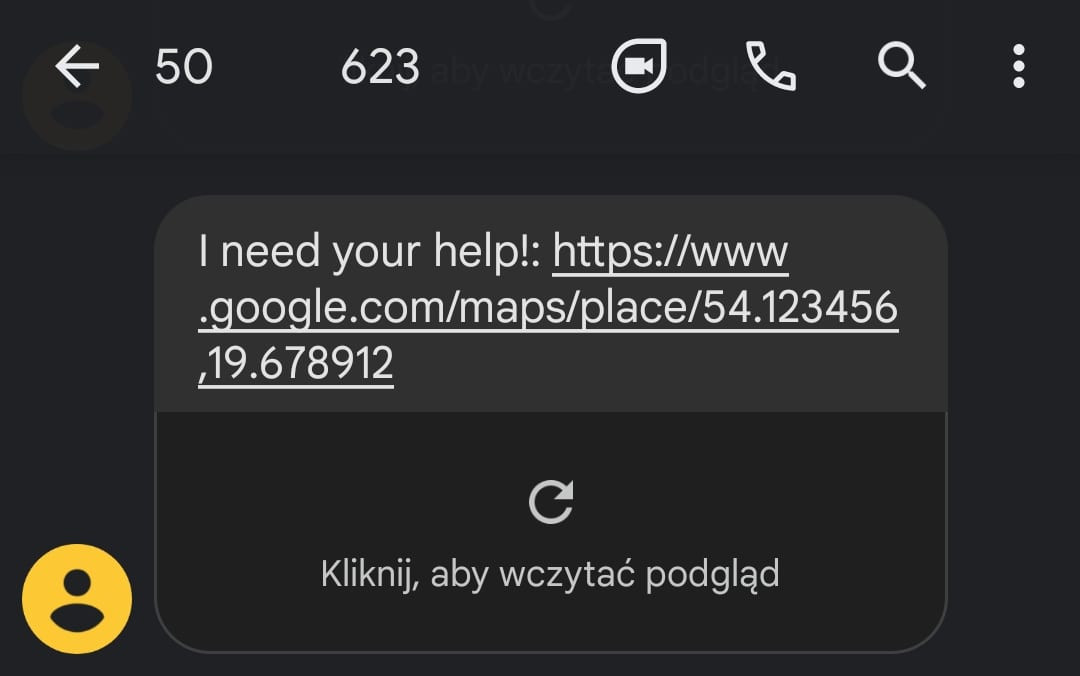
\includegraphics[width=6cm]{Graphics/sms.jpg}
    \caption{Odebrana wiadomość SMS z lokalizacją}
    \label{img:sms}
    \end{subfigure}%
    \vspace{1cm}
    \begin{subfigure}[b]{6cm}
    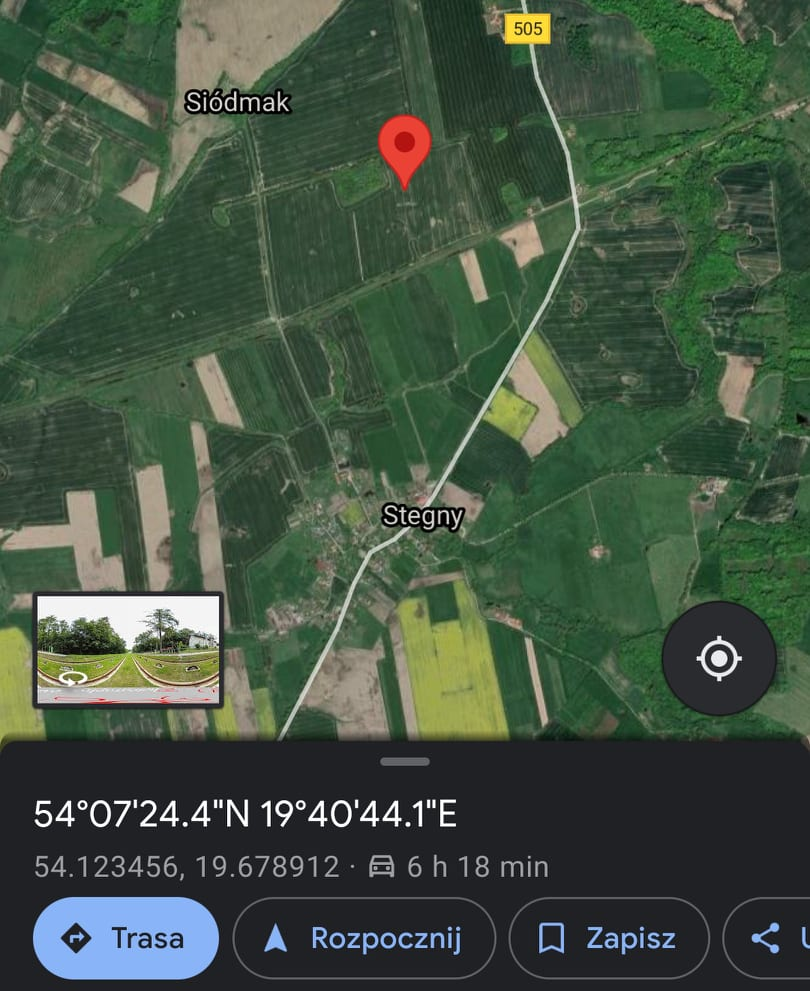
\includegraphics[width=6cm]{Graphics/maps.jpg}
    \caption{Lokalizacja na mapie Google}
    \label{img:maps}
    \end{subfigure}
    \caption{Wysyłane powiadomienie z lokalizacją}
    \label{img:notification}
\end{figure}